\documentclass[11pt,a4paper]{article}

\usepackage{../../templates/style}

\begin{document}

\begin{problem}{}{standard input}{standard output}{1 second}{16 megabytes}

เวลาเขียนโปรแกรมภาษา C เราสามารถเอาเนื้อหาของไฟล์หนึ่ง ๆเข้ามาใส่ในไฟล์อีกไฟล์หนึ่ง ได้ด้วยการใช้คำสั่ง #include ยกตัวอย่างเช่น ถ้า main.c และ lib.h มีเนื้อหาดังต่อไปนี้

\begin{figure}[h!]
\centering
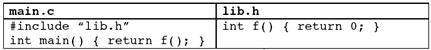
\includegraphics[width=0.7\textwidth]{../latex/img/1057/1057-1.png}
\end{figure}

เวลาคอมไพล์ คอมไพเลอร์ภาษา C จะเขียนเนื้อหาของ main.c ใหม่ โดยเอาเนื้อหาของ lib.h ไปแทรกไว้ที่คำสั่ง #include “lib.h” ใน main.c ดังนั้นเนื้อหาใหม่ของ main.c คือ

\begin{figure}[h!]
\centering
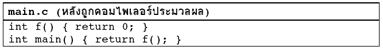
\includegraphics[width=0.7\textwidth]{../latex/img/1057/1057-2.png}
\end{figure}



อนึ่ง ในไฟล์ที่ถูกไฟล์อื่น include อาจมีคำาสั่ง #include อยู่ก็ได้ และในไฟล์หนี่งอาจมีการ include ไฟล์อื่น ๆมากกว่าหนึ่งไฟล์ได้ ยกตัวอย่างเช่น

\begin{figure}[h!]
\centering
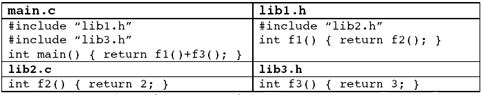
\includegraphics[width=0.7\textwidth]{../latex/img/1057/1057-3.png}
\end{figure}

จะได้ว่าเวลาคอมไพเลอร์ภาษา C จะเขียนเนื้อหาของ main.c ใหม่ ดังนี้

\begin{figure}[h!]
\centering
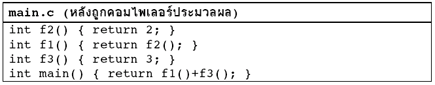
\includegraphics[width=0.7\textwidth]{../latex/img/1057/1057-4.png}
\end{figure}


อย่างไรก็ดีหากผู้เขียนโปรแกรมไม่ระมัดระวังก็อาจทำให้เกิดปัญหาได้สองประการคือ

1. ไฟล์เดียวกันถูก include มากกว่าหนึ่งครั้ง เช่น


\begin{figure}[h!]
\centering
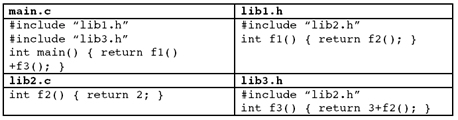
\includegraphics[width=0.7\textwidth]{../latex/img/1057/1057-5.png}
\end{figure}


ในกรณีเมื่อคอมไพเลอร์ทำการคอมไพล์ main.c ไฟล์ lib2.c จะถูก include สองครั้ง ครั้งหนึ่ง จากไฟล์ lib1.h และอีกครั้ง จาก lib3.h ซึ่ง ทำให้ฟังก์ชัน f2() ถูกนิยามสองครั้ง ซึ่ง อาจทำให้คอมไพล์ไม่ผ่านได้

2. ไฟล์ include กันเป็นวงกลม เช่น

\begin{figure}[h!]
\centering
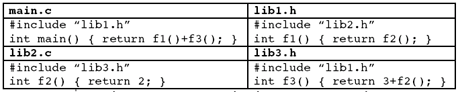
\includegraphics[width=0.7\textwidth]{../latex/img/1057/1057-6.png}
\end{figure}



สังเกตว่าเมื่อคอมไพเลอร์ภาษา C คอมไพล์ไฟล์ main.c แล้วไฟล์ lib1.h จะ include ไฟล์ lib2.h ซึ่ง include ไฟล์ lib3.h ซึ่ง include ไฟล์ lib1.h และสามารถวนไปเช่นนี้เรื่อย ๆโดยไม่จำกัด



\bigskip
\underline{\textbf{โจทย์}}  กำหนดไฟล์โปรแกรมภาษา C มาให้ $N$ ไฟล์ แต่ละไฟล์จะถูกระบุด้วยตัวเลขตั้ง แต่ $1$ ถึง $N$ พร้อมทัังข้อมูลว่าไฟล์ใด include ไฟล์ได้บ้าง จงเขียนโปรแกรมเพื่อตอบคำถามว่าสำหรับไฟล์ทุกๆ ไฟล์ เมื่อคอมไพเลอร์ภาษา C ทำาการคอมไพล์ไฟล์นั้น แล้วจะเกิดปัญหาใดปัญหาหนึ่ง ในสองปัญหาที่กล่าวถึงข้างบนหรือไม่

\InputFile

\textbf{บรรทัดแรก} รับค่าจำนวนเต็ม $N$ $(1 \leq N \leq 1\,000)$

\textbf{บรรทัดที่ $2$ ถึง $N+1$}  ในบรรทัดที่ $i+1$ (สำหรับทุก ๆ $1 \leq i \leq N$ ) บอกว่าไฟล์ $i$ ทำาการ include ไฟล์ใดบ้าง ซึ่งจะระบุในรูปแบบ $k$ $a_1$ $a_2$ $a_3$ $…$ $a_k$ โดยที่ $k$ และทุก ๆ $a_j$ ที่ $1 \leq j \leq k$ เป็นจำนวนเต็มที่ไม่เป็นลบและมีค่าไม่เกิน $N$ โดยบรรทัดดังกล่าวมีความหมายว่าไฟล์ $i$ ทำการ include ไฟล์ $a_1, a_2, …, a_k$ เรารับประกันว่าเลข $a_j$ จะมีค่าไม่ซ้ำกัน (ในไฟล์หนึ่ง ๆ จะไม่มีการ include ไฟล์เดียวกันซ้ำสองครั้ง ) และในบรรทัดที่ $i + 1$ จะไม่มี $a_j$ ใดๆ ที่มีค่าเท่ากับ $i$ (ไฟล์แต่ละไฟล์จะไม่ include ตัวเอง) นอกจากนี้รับประกันว่าจำนวนการ include ทั้ง หมดจะไม่เกิน $3\,000$ ครั้ง


\OutputFile

\textbf{มี $N$ บรรทัด} แต่ละบรรทัดมีข้อความ YES หรือ NO ถ้าเมื่อคอมไพเลอร์ภาษา C คอมไพล์ไฟล์ $i$ แล้วเกิดปัญหาใดปัญหาหนึ่งในปัญหาสองข้อข้างต้น ให้พิมพ์ YES ในบรรทัดที่ $i$ แต่ถ้าหากไม่เกิดปัญหาใดขึ้นเลยให้พิมพ์ NO


\Examples

\begin{example}
\exmp{2
1 2
0}{NO
NO}%
\exmp{3
1 2
1 3
1 1}{YES
YES
YES}%
\exmp{4
2 2 3
1 4
1 4
0}{YES
NO
NO
NO}%
\end{example}


\Source

Young Thai Online Programming Competition 2008

\end{problem}

\end{document}